%% It is just an empty TeX file.
%% Write your code here.


\documentclass{article}

\usepackage{graphicx}

\usepackage{pdfpages}



\title{RSA}


\begin{document}             % End of preamble and beginning of text.

\maketitle                   % Produces the title.




\section{RSA}

\subsection{Introduction}

There are many applications for RSA, but in practice it is most often used for:

\begin{itemize}
    \item  encryption of small pieces of data, especially for key transport
    \item  digital signatures, digital certificates onthe Internet
\end{itemize}
 
However, it should be noted that RSA encryption is not meant to replace symmetric ciphers because it is several times slower than ciphers such as AES. This is because of the many computations involved in performing RSA (or any other pub-key algorithm) as we learn later in this chapter. Thus, the main use of the encryption feature is to securely exchange a key for a symmetric cipher (key transport). In practice, RSA is often used together with a symmetric cipher such as AES, where the symmetric cipher does the actual bulk data encryption.
 

\subsection{Encryption and Decryption}

%%\includegraphics[scale=.1]{dark-wallpaper-36.jpg}




%%somethinghere



\subsection{Keygeneration and proof of correctness}

\subsubsection{Key Generation steps}

 Output: public key: kpub = (n,e) and private key: kpr = (d)

1. Choose two large primes p and q.

2. Compute n = p · q.

3. Compute \(\phi(n)= (p - 1)(q-1)\).

4. Select the public exponent e ∈ \{1,2,...,\phi(n) - 1\} such that gcd(e,\phi(n)) = 1.

5. Compute the private key d such that d · e ≡ mod\phi(n)

\subsubsection{proof of correctness}

Proof.


We need to show that decryption is the inverse function of encryption,
dkpr(ekpub (x)) = x.


We start with the construction rule for the public and private
key: \(d.e \equiv 1 mod \phi(n)\).

By definition of the modulo operation, this is equivalent to:
\(d·e = 1+t ·\phi(n)\),where t is some integer.

Inserting this expression in Eq.:
dkpr(y) \equiv x^{de} \equiv x^{(1+t·\phi(n))} \equiv x^{(t·\phi(n))}·x^1 \equiv \((x^{(\phi(n)t)})·x mod n\).
This means we have to prove that x \equiv {(x^\phi(n)t)} · x mod n.(7.4)


We use now Euler’s Theorem, which states that if gcd(x,n) = 1 then 1 \equiv \(x^{\phi(n)}\)mod n.

A minor generalization immediately follows:
1 \equiv 1^t \equiv \(x^{\phi(n).t}\) mod n, (7.5)

where t is any integer. For the proof we distinguish two cases:
First case: gcd(x,n) = 1
Euler’s Theorem holds here and we can insert Eq. (7.5) into (7.4):
dkpr(y) \equiv (x^{\phi(n)})^t · x \equiv 1 · x \equiv x mod n. 

\subsection{RSA Padding}



What we described so far is the so-called “schoolbook RSA” system which has several weaknesses. In practice RSA has to be used with a padding scheme. Padding
schemes are extremely important, and if not implemented properly, an RSA implementation may be insecure. The following properties of schoolbook RSA encryption
are problematic:
\begin{itemize}
     

 
 \item RSA encryption is deterministic, i.e., for a specific key, a particular plaintext
is always mapped to a particular ciphertext. An attacker can derive statistical
properties of the plaintext from the ciphertext. Furthermore, given some pairs
of plaintext–ciphertext, partial information can be derived from new ciphertexts
which are encrypted with the same key.
 
 \item Plaintext values x = 0, x = 1, or x = −1 produce ciphertexts equal to 0, 1, or −1.
 
 \item Small public exponents e and small plaintexts x might be subject to attacks if
no padding or weak padding is used. However, there is no known attack against
small public exponents such as e = 3.
\end{itemize}
RSA has another undesirable property, namely that it is malleable. A crypto
scheme is said to be malleable if the attacker Oscar is capable of transforming the ciphertext into another ciphertext which leads to a known transformation of the plaintext. Note that the attacker does not decrypt the ciphertext but is merely capable of
manipulating the plaintext in a predictable manner. This is easily achieved in the
case of RSA if the attacker replaces the ciphertext y by se y, where s is some integer.
If the receiver decrypts the manipulated ciphertext, he computes:


(s^(e) y)^d \equiv s^{ed} x^{ed} \equiv sx mod n.



Even though Oscar is not able to decrypt the ciphertext, such targeted manipulations
can still do harm. For instance, if x were an amount of money which is to be transferred or the value of a contract, by choosing s = 2 Oscar could exactly double the
amount in a way that goes undetected by the receiver.
A possible solution to all these problems is the use of padding, which embeds a random structure into the plaintext before encryption and avoids the above
mentioned problems. Modern techniques such as Optimal Asymmetric Encryption
Padding (OAEP) for padding RSA messages are specified and standardized in Public Key Cryptography Standard #1 (PKCS #1).

\section{Attacks}

There have been numerous attacks proposed against RSA since it was invented in
1977. None of the attacks are serious, and moreover, they typically exploit weaknesses in the way RSA is implemented or used rather than the RSA algorithm itself.
There are three general attack families against RSA:


1. Protocol attacks


2. Mathematical attacks


3. Side-channel attacks


We comment on each of them in the following



\subsection{Protocol Attacks}


Protocol attacks exploit weaknesses in the way RSA is being used. There have been
several protocol attacks over the years. Among the better known ones are the attacks
that exploit the malleability of RSA, which was introduced in the previous section.
Many of them can be avoided by using padding. Modern security standards describe
exactly how RSA should be used, and if one follows those guidelines, protocol
attacks should not be possible.


\subsection{Mathematical Attacks}

The best mathematical cryptanalytical method we know is factoring the modulus.
An attacker, Oscar, knows the modulus n, the public key e and the ciphertext y. His
goal is to compute the private key d which has the property that e · d \equiv mod\phi(n).

It seems that he could simply apply the extended Euclidean algorithm and compute d. 
However, he does not know the value of \phi(n). 

At this point factoring comes in:

the best way to obtain this value is to decompose n into its primes p and q. 
If Oscar can do this, the attack succeeds in three steps:


\phi(n)=(p−1)(q−1)


d^(−1) \equiv e mod \phi(n)


x \equiv y^d mod n.


In order to prevent this attack, the modulus must be sufficiently large. This is the
sole reason why moduli of 1024 or more bit are needed for a RSA. The proposal of
the RSA scheme in 1977 sparked much interest in the old problem of integer factorization. In fact, the major progress that has been made in factorization in the last
three decades would most likely not have happened if it weren’t for RSA. Table 7.3
shows a summary of the RSA factoring records that have occurred since the beginning of the 1990s. These advances have been possible mainly due to improvements
in factoring algorithms, and to a lesser extent due to improved computer technology.

Even though factoring has become easier than the RSA designers had assumed 30
years ago, factoring RSA moduli beyond a certain size still is out of reach.


\subsection{Side-Channel Attacks}



A third and entirely different family of attacks are side-channel attacks. They exploit
information about the private key which is leaked through physical channels such as
the power consumption or the timing behavior. In order to observe such channels, an
attacker must typically have direct access to the RSA implementation, e.g., in a cell
phone or a smart card

\subsection{Lesson Learned}
\begin{itemize}

\item the most widely used public-key cryptosystem. In the future, elliptic
curve cryptosystems will probably catch up in popularity.
 RSA is mainly used for key transport (i.e., encryption of keys) and digital signatures.
 \item 
 The public key e can be a short integer. The private key d needs to have the
full length of the modulus. Hence, encryption can be significantly faster than
decryption.
\item 
 RSA relies on the integer factorization problem. Currently, 1024-bit (about 310
decimal digits) numbers cannot be factored. Progress in factorization algorithms
and factorization hardware is hard to predict. It is advisable to use RSA with
a 2048-bit modulus if one needs reasonable long-term security, especially with
respect to extremely well funded attackers.
\item 
 “Schoolbook RSA” allows several attacks, and in practice RSA should be used
together with Padding
\end{itemize}



\subsection{From the lecture and exercise solution}


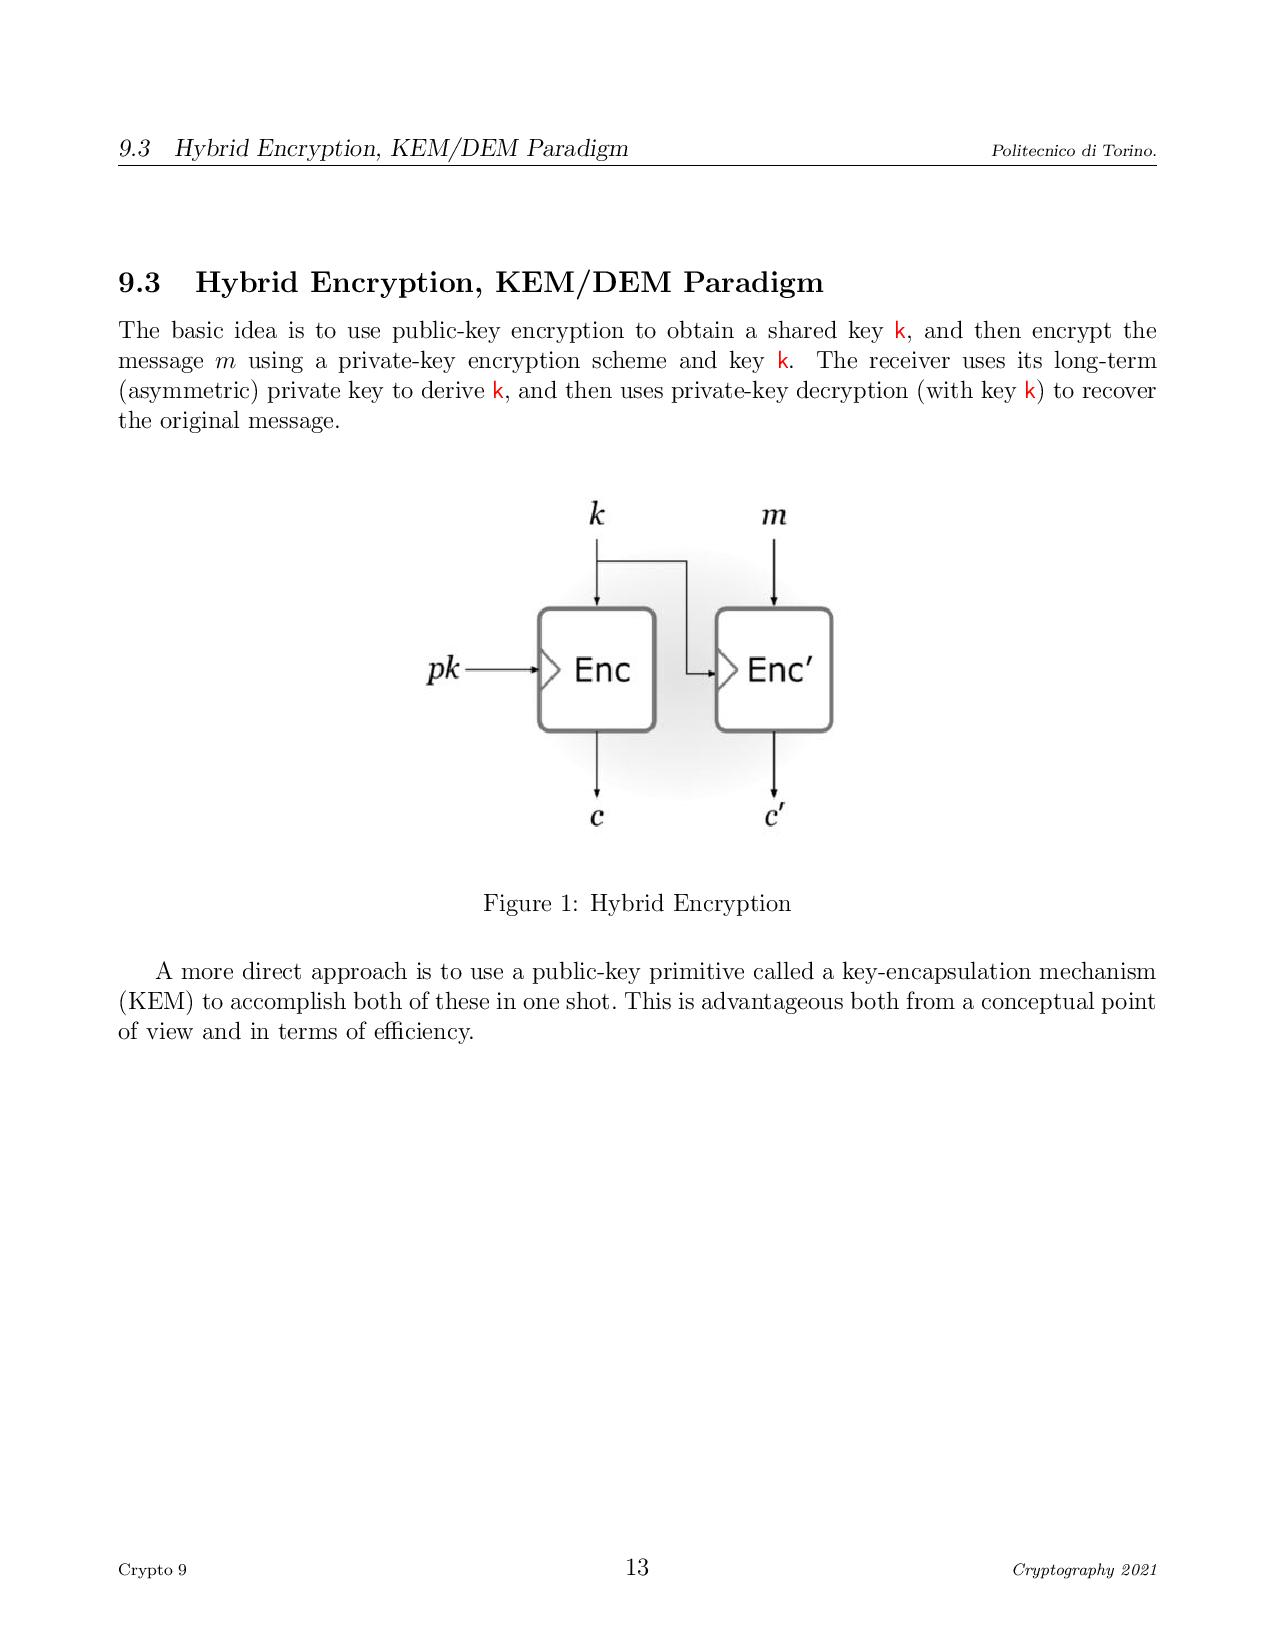
\includegraphics[scale=.7]{Crypto9-13-page-001.jpg}


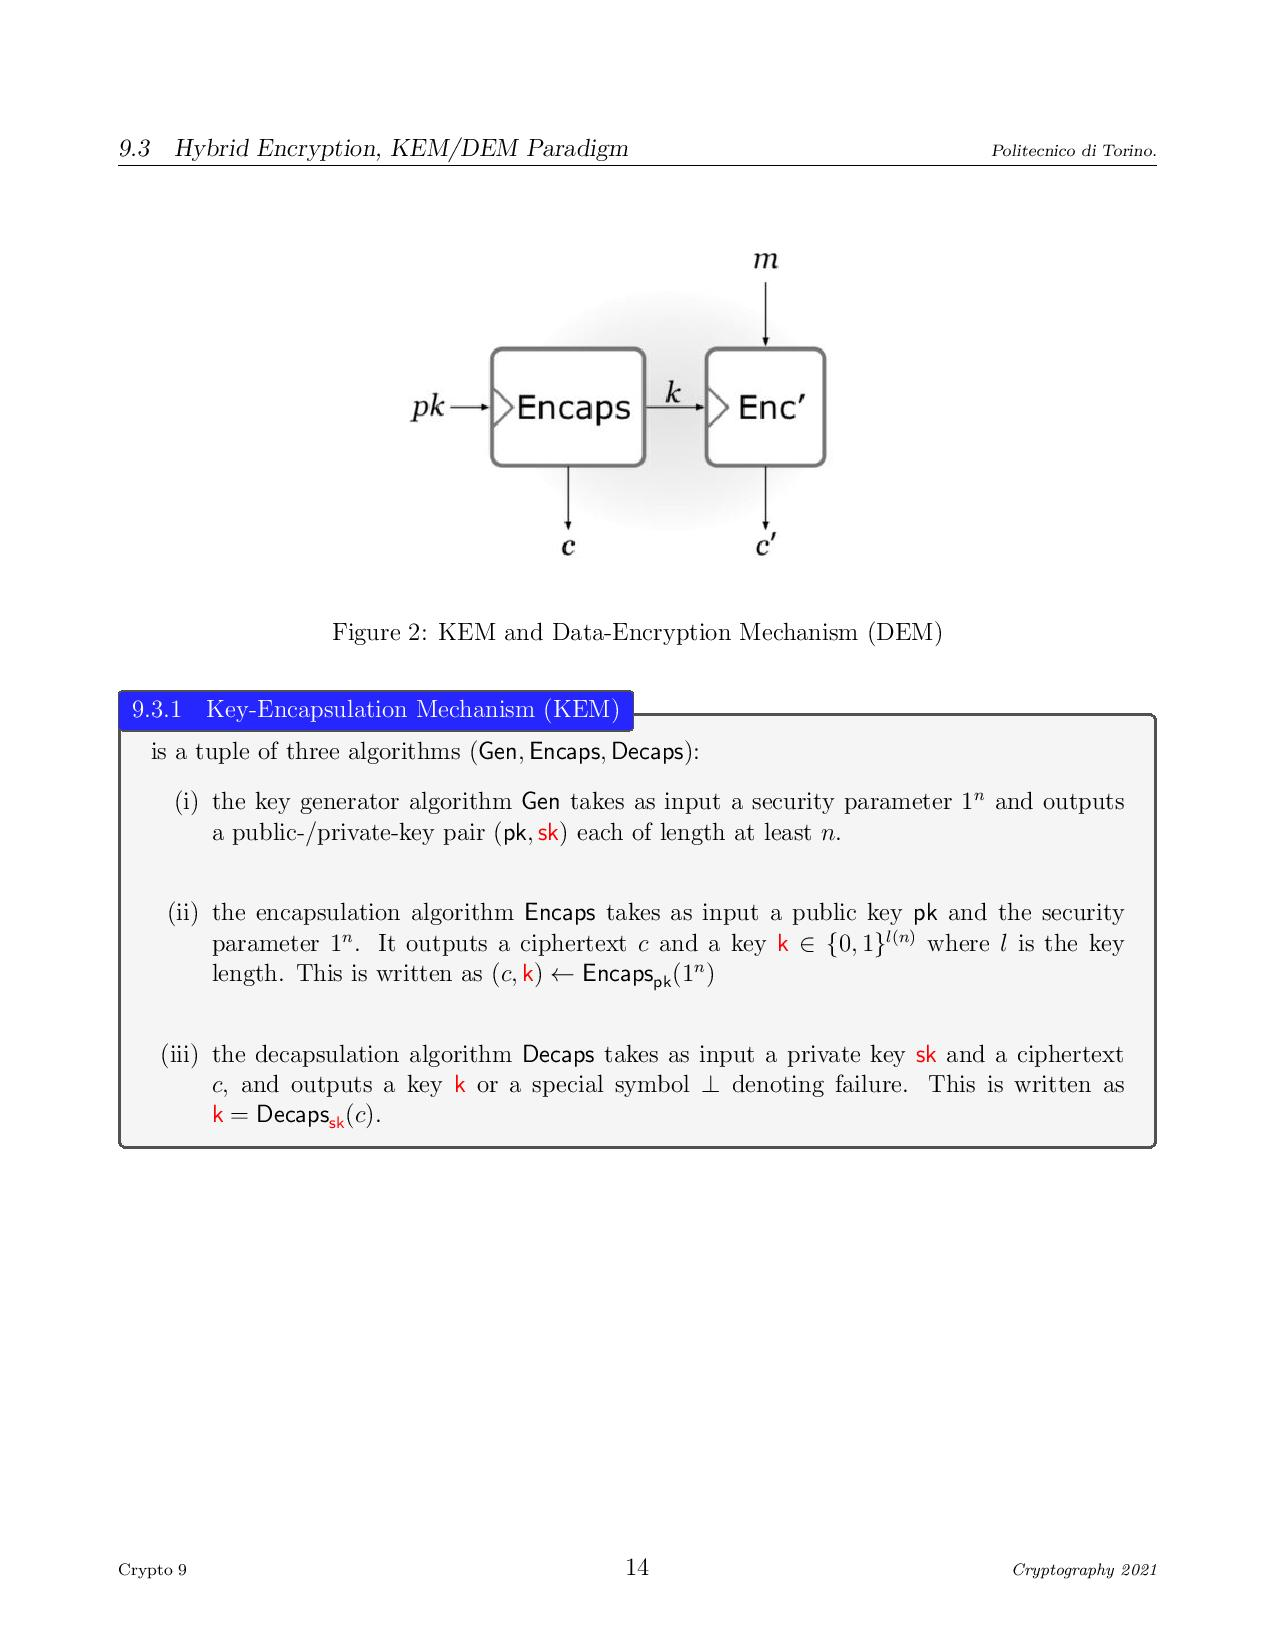
\includegraphics[scale=.7]{Crypto9-14-page-001.jpg}








\includegraphics[scale=.1, angle=-90]{IMG_20210521_120201.jpg}


\vspace{10 mm}


\includegraphics[scale=.1, angle=-90]{IMG_20210521_120211_1.jpg}


\url https://www.di-mgt.com.au/crt.html











\end{document}   
%% Write your code here.







